\documentclass{sig-alternate}

\begin{document}

\title{Buscando la temperatura ideal}

\numberofauthors{2}

\author{
    \alignauthor
    Abramowicz, Pablo\\
    \email{pabramow@alu.itba.edu.ar} \\
    \ \\
    Gomez Vidal, Maximiliano\\
    \email{dgomezvi@alu.itba.edu.ar} \\
    \alignauthor
    Sessa, Carlos\\
    \email{csessa@alu.itba.edu.ar} \\
    \ \\
    Villa Fern\'{a}ndez, Santiago\\
    \email{svillafe@alu.itba.edu.ar} \\
}

\maketitle

\begin{abstract}
En este art\'{i}culo se comparan dos modelos alternativos para el 
calefaccionamiento de un edificio, teniendo en cuenta fac\-to\-res determinantes 
tales como la amplitud t\'{e}rmica y el consumo energ\'{e}tico. Se realizan 
simulaciones para cada uno de los mismos.
\end{abstract}

\keywords{Calefacci\'{o}n, consumo energ\'{e}tico, simulaci\'{o}n, temperatura 
ideal, climatizaci\'{o}n}

\section{Introducci\'{o}n}\label{introduccion}

Se desea escoger una estrategia para el calefaccionamiento de un
edificio. Para llevar a cabo esta tarea resulta fundamental estudiar c\'{o}mo 
var\'{i}a la temperatura en el interior del mismo. Se considera que este sistema 
din\'{a}mico es continuo y determinista, por lo que puede ser modelado mediante 
una ecuaci\'{o}n diferencial.

Se presentan dos modelos para este sistema. En ambos casos se establece que
la temperatura del exterior del edificio en esa \'{e}poca del a\~{n}o
var\'{i}a de acuerdo a 

\begin{equation}
\label{t_exterior}
T_{out} (t) = 10 - 6 \cos\frac{2 \pi t}{24}.
\end{equation}

En la secci\'{o}n \ref{modelosysimulaciones} se presentan ambos modelos y
se de\-sa\-rro\-llan las simulaciones correspondientes.
En la secci\'{o}n \ref{resultados} se analizan y contrastan los resultados
obtenidos en las simulaciones.
En la secci\'{o}n \ref{conclusiones} se establecen las conclusiones y se
escoge el modelo m\'{a}s conveniente.

\section{Modelos y simulaciones}\label{modelosysimulaciones}

\subsection{Modelo 1}

\subsubsection{Descripci\'{o}n}

Se propone un primer modelo en donde la variaci\'{o}n de la temperatura interior
del edificio var\'{i}a al ritmo dictado por la ecuaci\'{o}n

\begin{equation}
\label{t_primer_modelo}
\frac{dT}{dt} = k ( T_{out} - T ) + k_{u} ( T^{*} - T )
\end{equation}

donde $T_{out}$ representa la temperatura exterior, $T^{*}$ la temperatura
fijada por un sistema de aire acondicionado y $k$, $k_{u}$ son constantes
de enfriamiento.

A partir de la ecuaci\'{o}n (\ref{t_primer_modelo}) se observa que existen dos
factores esenciales para determinar la temperatura en el interior del edificio.
El t\'{e}rmino que involucra a $k$ indica como se
transfiere el calor externo hacia el interior del edificio, siendo $k$ el
coeficiente de transferencia. Por otra parte, el t\'{e}rmino que contiene a $k_{u}$
 determina la ganancia o p\'{e}rdida de calor debida a la configuraci\'{o}n del 
sistema de aire acondicionado. \\
Si la temperatura $T^{*}$ se fija de modo que 

\begin{equation}
\label{t_fijada}
k ( \overline{T}_{out} - T_{D})
+ k_{u} ( T^{*} - T_{D} ) = 0
\end{equation}
para una temperatura interior deseada $T_{D}$,
donde $\overline{T}_{out}$ es la temperatura exterior media, entonces la
ecuaci\'{o}n (\ref{t_primer_modelo}) puede escribirse de la siguiente manera

\begin{equation}
\label{t_primer_modelo_modificada}
\frac{dT}{dt} = k ( T_{out} - \overline{T}_{out} ) + ( k + k_{u} ) ( T_{D} - T )
\end{equation}

Partiendo de la ecuaci\'{o}n (\ref{t_fijada}) se establece la igualdad

\begin{equation}
T^{*}=\frac{-k\left(\bar{T}_{out}-T_{D}\right)}{k_{u}}+T_{D}
\end{equation} 
 
que al reemplazarse en (\ref{t_primer_modelo}) da por resultado la expresi\'{o}n
\begin{equation}
\frac{dT}{dt}=k(T_{out}-T)+k_{u}\left(\frac{-k\left(\bar{T}_{out}-T_{D}\right)}{k_{u}}+T_{D}-T\right)
\end{equation}

Reordenando y agrupando se obtiene la expresi\'{o}n dada en (\ref
{t_primer_modelo_modificada}).

\subsubsection{Simulaci\'{o}n}

Se desea estudiar el comportamiento del sistema durante $48$ horas para una
tem\-pe\-ra\-tu\-ra deseada $T_{D} = 20^{\circ}$. Se establece
$k_{u} = 0.70^\circ$  hora$^{-1}$ y se hace variar el coeficiente de transferencia
$k$ tomando los valores $0.25, 0.5, 1,$
$2, 5, 10, 15$ y $20$ hora$^{-1}$.

Como temperatura inicial dentro del edificio se toma la media de la
tem\-pe\-ra\-tu\-ra exterior.

En la Figura $1$ se observa que la temperatura en 
el interior del edificio presenta oscilaciones. Adem\'{a}s, dichas oscilaciones
aumentan su amplitud a medida que se incrementa el coeficiente $k$, indicando
que la influencia de la tem\-pe\-ra\-tu\-ra exterior se hace mayor hasta
gobernar por completo la temperatura del interior del edificio.

\subsubsection{Consideraciones energ\'{e}ticas}

La energ\'{i}a que se consume para calefaccionar el edificio durante $48$
horas resulta

\begin{equation}
\label{energia_primer_modelo}
E_{1} = \int_{0}^{48} k_{u} | T^{*} - T | dt
\end{equation}

El resultado arrojado al utilizar el m\'{e}todo de Euler para integrar 
num\'{e}ricamente la expresi\'{o}n (\ref{energia_primer_modelo}) es un 
consumo e\-ner\-g\'{e}\-ti\-co de aproximadamente $130J$.

\subsection{Modelo 2}

\subsubsection{Descripci\'{o}n}

Como segunda alternativa se propone un modelo m\'{a}s realista,
dado por

\begin{equation}
\label{segundo_modelo}
\frac{dT}{dt} = k ( T_{out} - T ) + u
\end{equation}

siendo $u$ la funci\'{o}n que cumple

\begin{equation}
\label{u_segundo_modelo}
u =  \begin{cases} 4^{\circ} C h^{-1}, & \mbox{si }  T < T_{D} \\
-1^{\circ} C h^{-1}, & \mbox{si }  T > T_{D} + 1 \\
0, & \mbox{si }  T_{D} <= T <= T_{D}+1 \end{cases}
\end{equation}

La ecuaci\'{o}n (\ref{u_segundo_modelo}) muestra que el aporte del
sistema de aire acondicionado var\'{i}a de acuerdo a la temperatura
deseada en el interior del edificio y la temperatura real del mismo.

\subsubsection{Simulaci\'{o}n}

En la Figura $2$ se observa el comportamiento
de la temperatura en el interior del edificio cuando el coeficiente de transferencia
se fija en $k = 0.25^{\circ}$ hora$^{-1}$.

Se observa que en todo momento se mantiene una temperatura bastante pr\'{o}xima
a la deseada, sufriendo peque\~{n}as variaciones y presentando una amplitud
t\'{e}rmica de unos pocos grados cent\'{i}grados.

\begin{figure*}[hp]
\label{primer_modelo_variar_k}
\centering
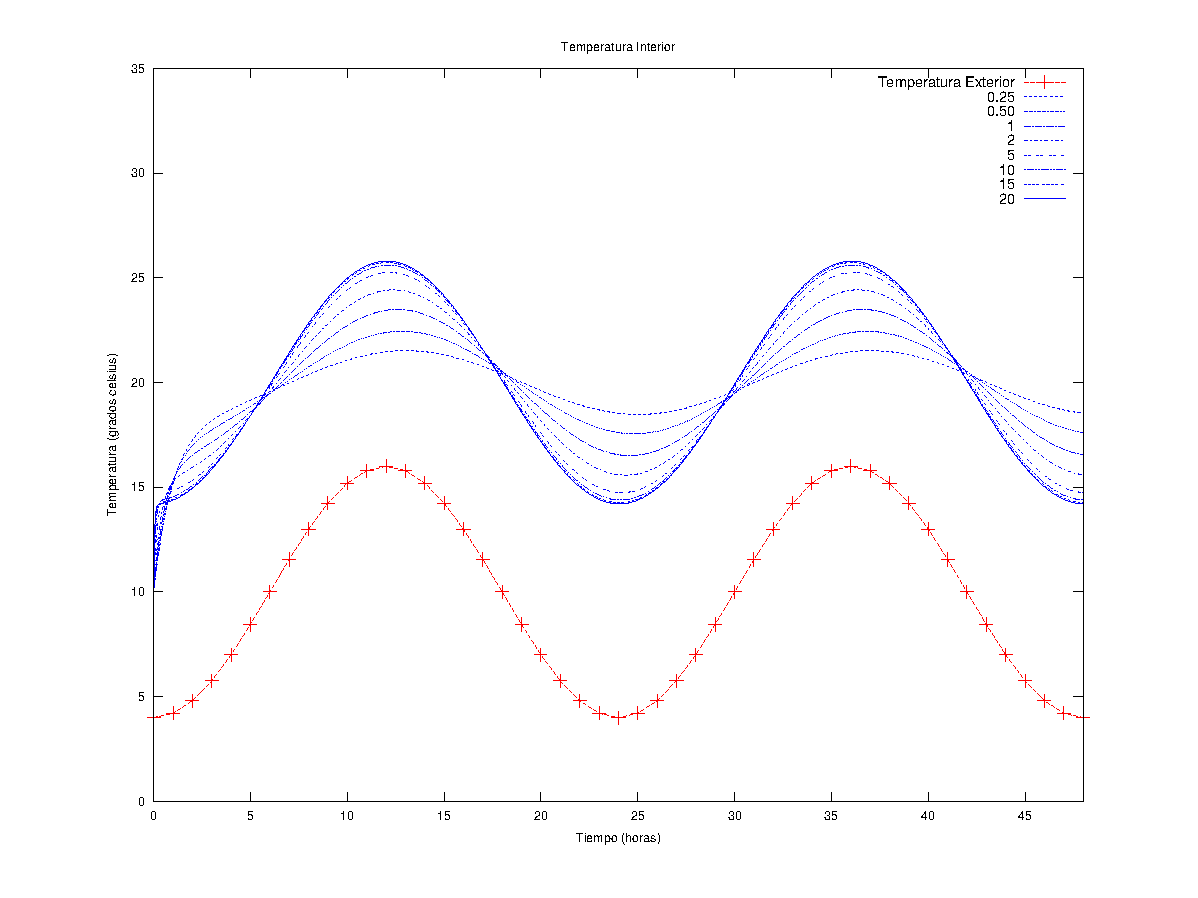
\includegraphics[scale=.8]{graficos/ej1b}
\caption{Modelo 1 - temperatura interior al variar $k$}
\end{figure*}

\begin{figure*}[hp]
\label{segundo_modelo_k_un_cuarto}
\centering
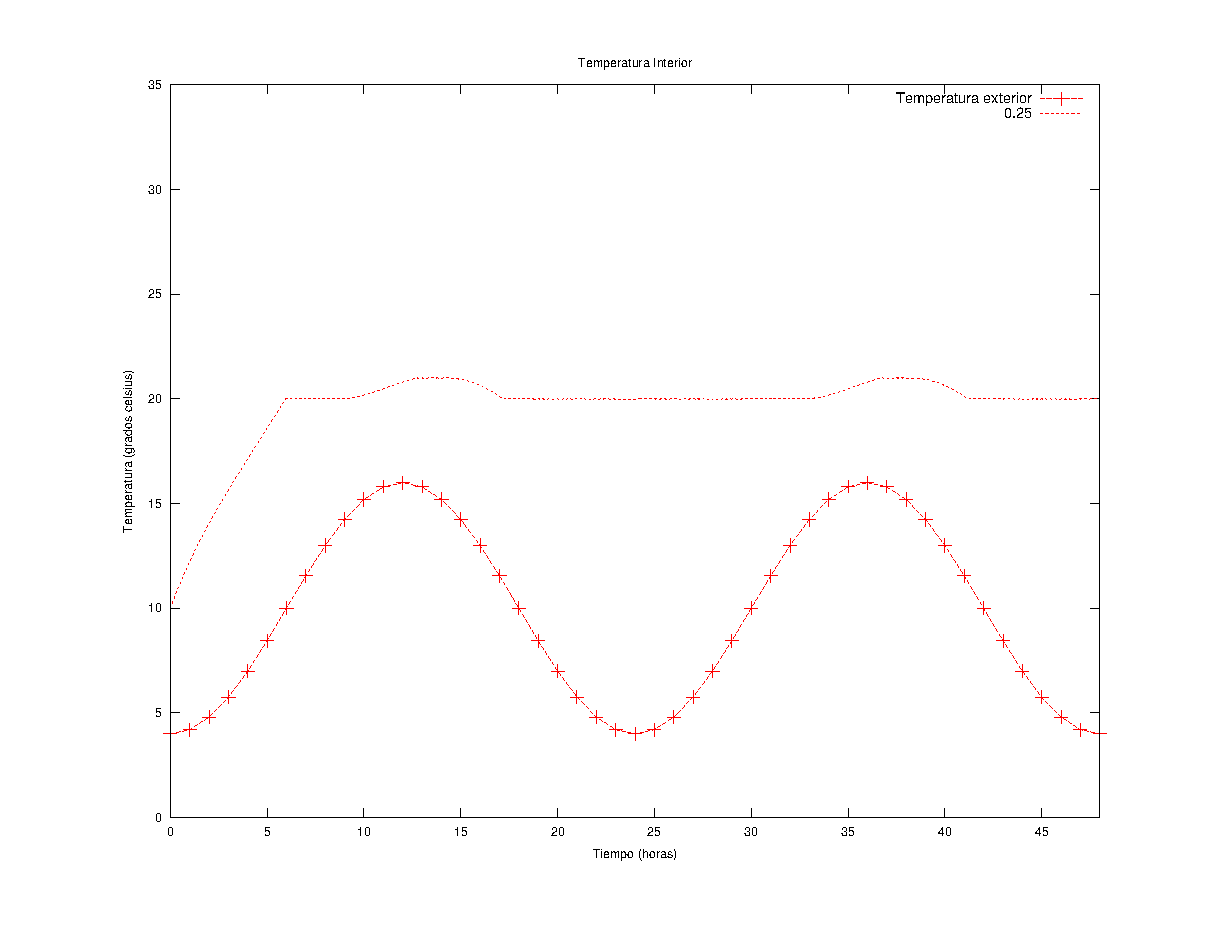
\includegraphics[scale=0.8]{graficos/modelo2}
\caption{Modelo 2 - Temperatura interior}
\end{figure*}

\subsubsection{Consideraciones energ\'{e}ticas}

La energ\'{i}a consumida para la calefacci\'{o}n del edificio durante $48$ horas
est\'{a} dada por

\begin{equation}
\label{energia_segundo_modelo}
E_{2} = \int_{0}^{48} | u | dt
\end{equation}

La integraci\'{o}n num\'{e}rica de esta expresi\'{o}n por el m\'{e}todo de
Euler muestra un consumo energ\'{e}tico total de alrededor de $122J$.

\section{Comparaci\'{o}n de resultados}\label{resultados}

En la Figura $3$ se muestra c\'{o}mo var\'{i}a 
la temperatura en el interior del edificio para ambos modelos. Se observa
que para valores de $k$ m\'{a}s grandes el Modelo 1 presenta se\-ve\-ras
fluctuaciones de temperatura, mientras que el Modelo 2 mantiene oscilaciones
de peque\~{n}a amplitud. Cabe destacar que el sistema descripto por el Modelo 2 
se estabiliza con una mayor velocidad que el dado por el Modelo 1.

\begin{figure*}[hp]
\label{comparacion_temp_interior}
\centering
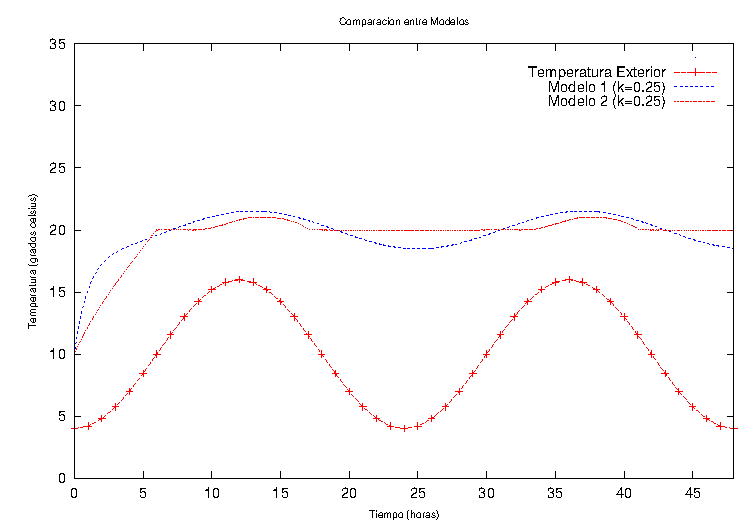
\includegraphics[scale=1.05]{graficos/ej1c}
\caption{Comparaci\'{o}n de la temperatura interior}
\end{figure*}

\begin{figure*}[hp]
\label{amplitud_termica}
\centering
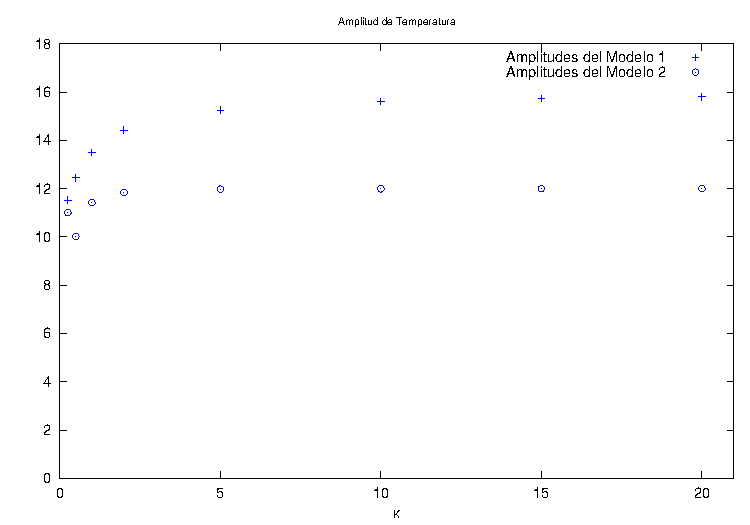
\includegraphics[scale=1.05]{graficos/amplitudes}
\caption{Amplitud t\'{e}rmica}
\end{figure*}

En lo que respecta al consumo de energ\'{i}a ambos modelos presentan
magnitudes similares, como se observa en las fi\-gu\-ras $5$ y 
$6$, resultando el consumo de la primera estrategia
levemente superior.

\begin{figure*}[hp]
\label{consumo_energia}
\centering
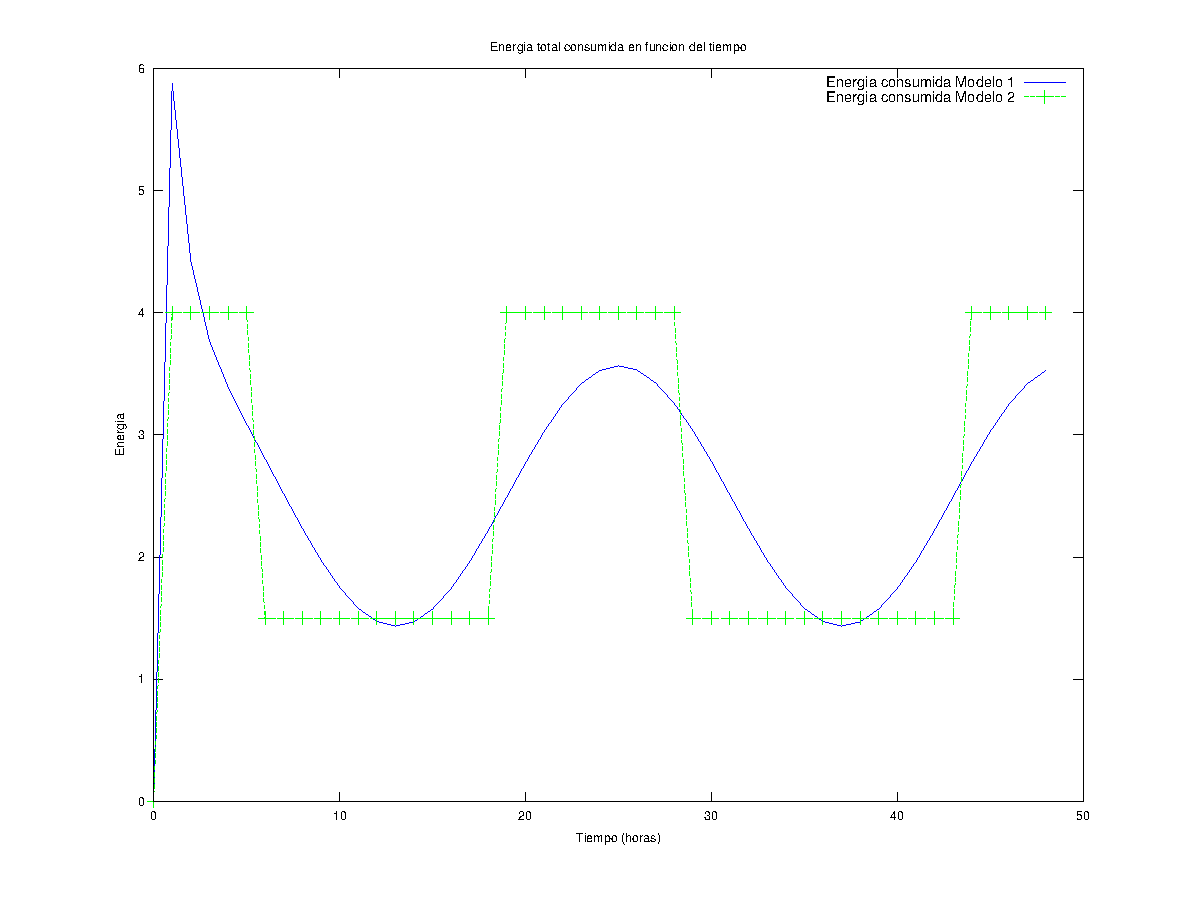
\includegraphics[scale=.8]{graficos/energia}
\caption{Consumo de energ\'{i}a}
\end{figure*}

\begin{figure*}[hp]
\label{consumo_energia_total}
\centering
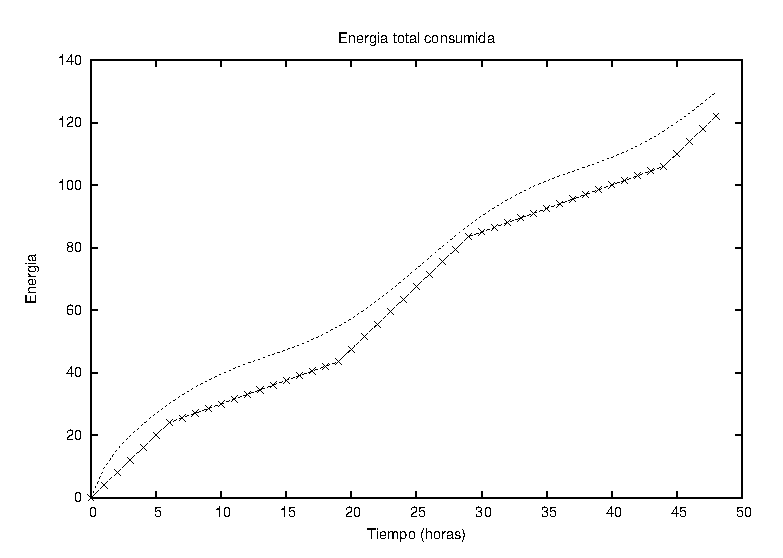
\includegraphics[scale=.8]{graficos/energiatotal}
\caption{Consumo total de energ\'{i}a}
\end{figure*}


\section{Conclusiones}\label{conclusiones}

Existen diversas maneras de modelar un sistema de calefaccionamiento para un
edificio. Para evaluar las distintas estrategias se deben tener en cuenta
factores cr\'{i}ticos tales como la amplitud t\'{e}rmica, el consumo
energ\'{e}tico y el tiempo que el sistema tarda en volverse estable.

En lo que respecta al consumo energ\'{e}tico el primer mo\-de\-lo posee un consumo
levemente mayor, aunque la pro\-xi\-mi\-dad en las magnitudes de ambos modelos
hace que este par\'{a}metro no resulte crucial para la elecci\'{o}n de uno por sobre
el otro.

El factor determinante en este caso es la amplitud t\'{e}rmica, que en definitiva
es la que determinar\'{a} el confort en el interior del edificio. El Modelo 2
resulta sumamente superior en este aspecto, manteniendo una temperatura muy
cercana a la deseada en todo momento y alcanzando su estado estacionario
en un tiempo muy breve.

\end{document}
